\chapter{Testovací laboratoř v praxi}

Nyní je všechna softwarová část testovací laboratoře připravena k použití a je potřeba vše začít testovat na fyzickém hardwaru. Pro osazení všech částí testovací laboratoře byl vytvořen speciální stojan. Stojan má ve spodní části poličky na různá vybavení. V poličkách je prozatím umístěn testovací server a konfigurovatelný switch. Horní část stojanu tvoří DIN lišty sloužící k umístění testovaných zařízení. Celkem je zde umístěno deset DIN lišt po dvou metrech. Pro jednodušší vedení kabeláže jsem na stojan připevnil plastové ranžírovací panely.

\begin{figure}[h]
  \centering
  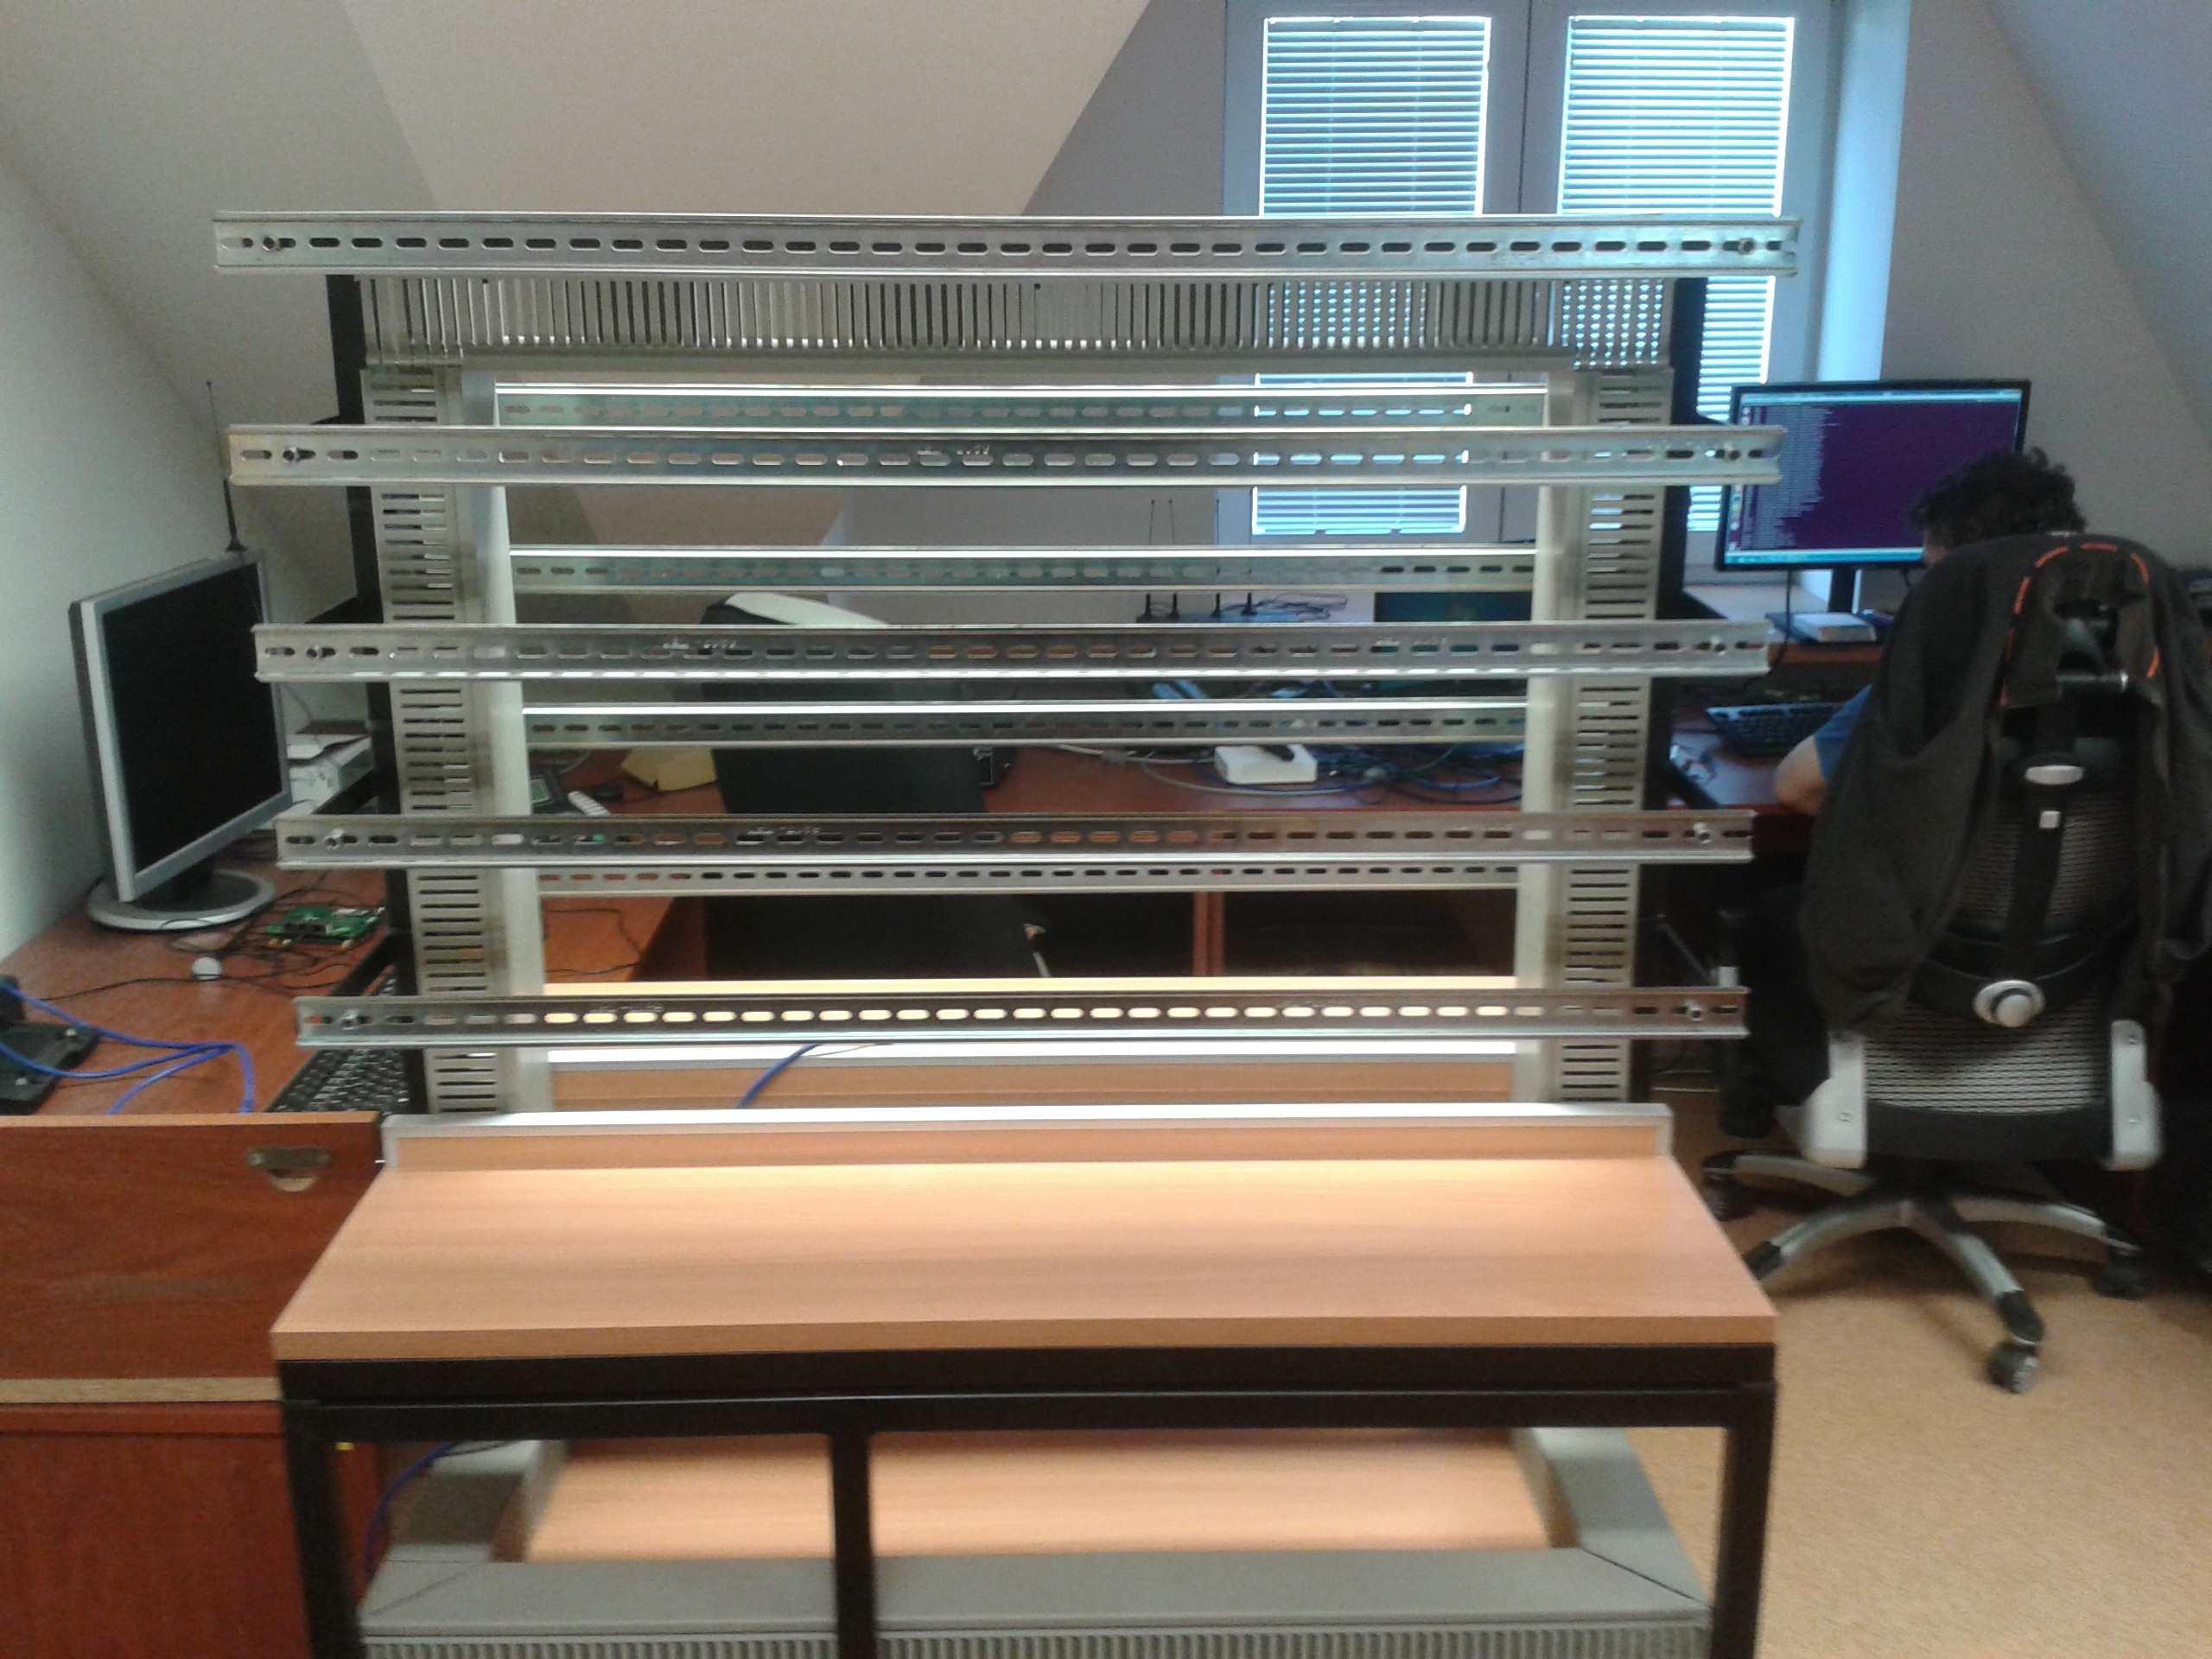
\includegraphics[width=\LW]{stojan1}
  \caption{Neosazený stojan}
  \label{fig:stojan1}
\end{figure}

Pro první fázi nasazení testování budu muset rozvést napájení a LAN síť. Napájení jsem řešil pomocí jednoho spínaného zdroje s možností montování na DIN lištu. Samotný zdroj má pouze dvě svorky na výstupní napájení, tudíž jsem vedle zdroje umístil svorkovnice na DIN lištu pro rozvedení napájení všech třiceti testovaných zařízení. Napájecí kabely  testovaných zařízení jsou dále vedeny ranžírovacím panelem a rovnoměrně po celé délce stojanu vyvedeny ven. Ethernetové kabely jsem vedl od switche umístěného ve střední polici stojanu do~svrchního ranžírovacího panelu, kde jsou Ethernetové kabely také rovnorměrně vyvedeny ven. Tímto rozložením jsem vytvořil univerzální stojan, kde pro připojení nového zařízení stačí pouze zařízení připevnit na DIN lištu, připojit napájení a Ethernet pomocí volně visících kabelů.

\begin{figure}[h]
  \centering
  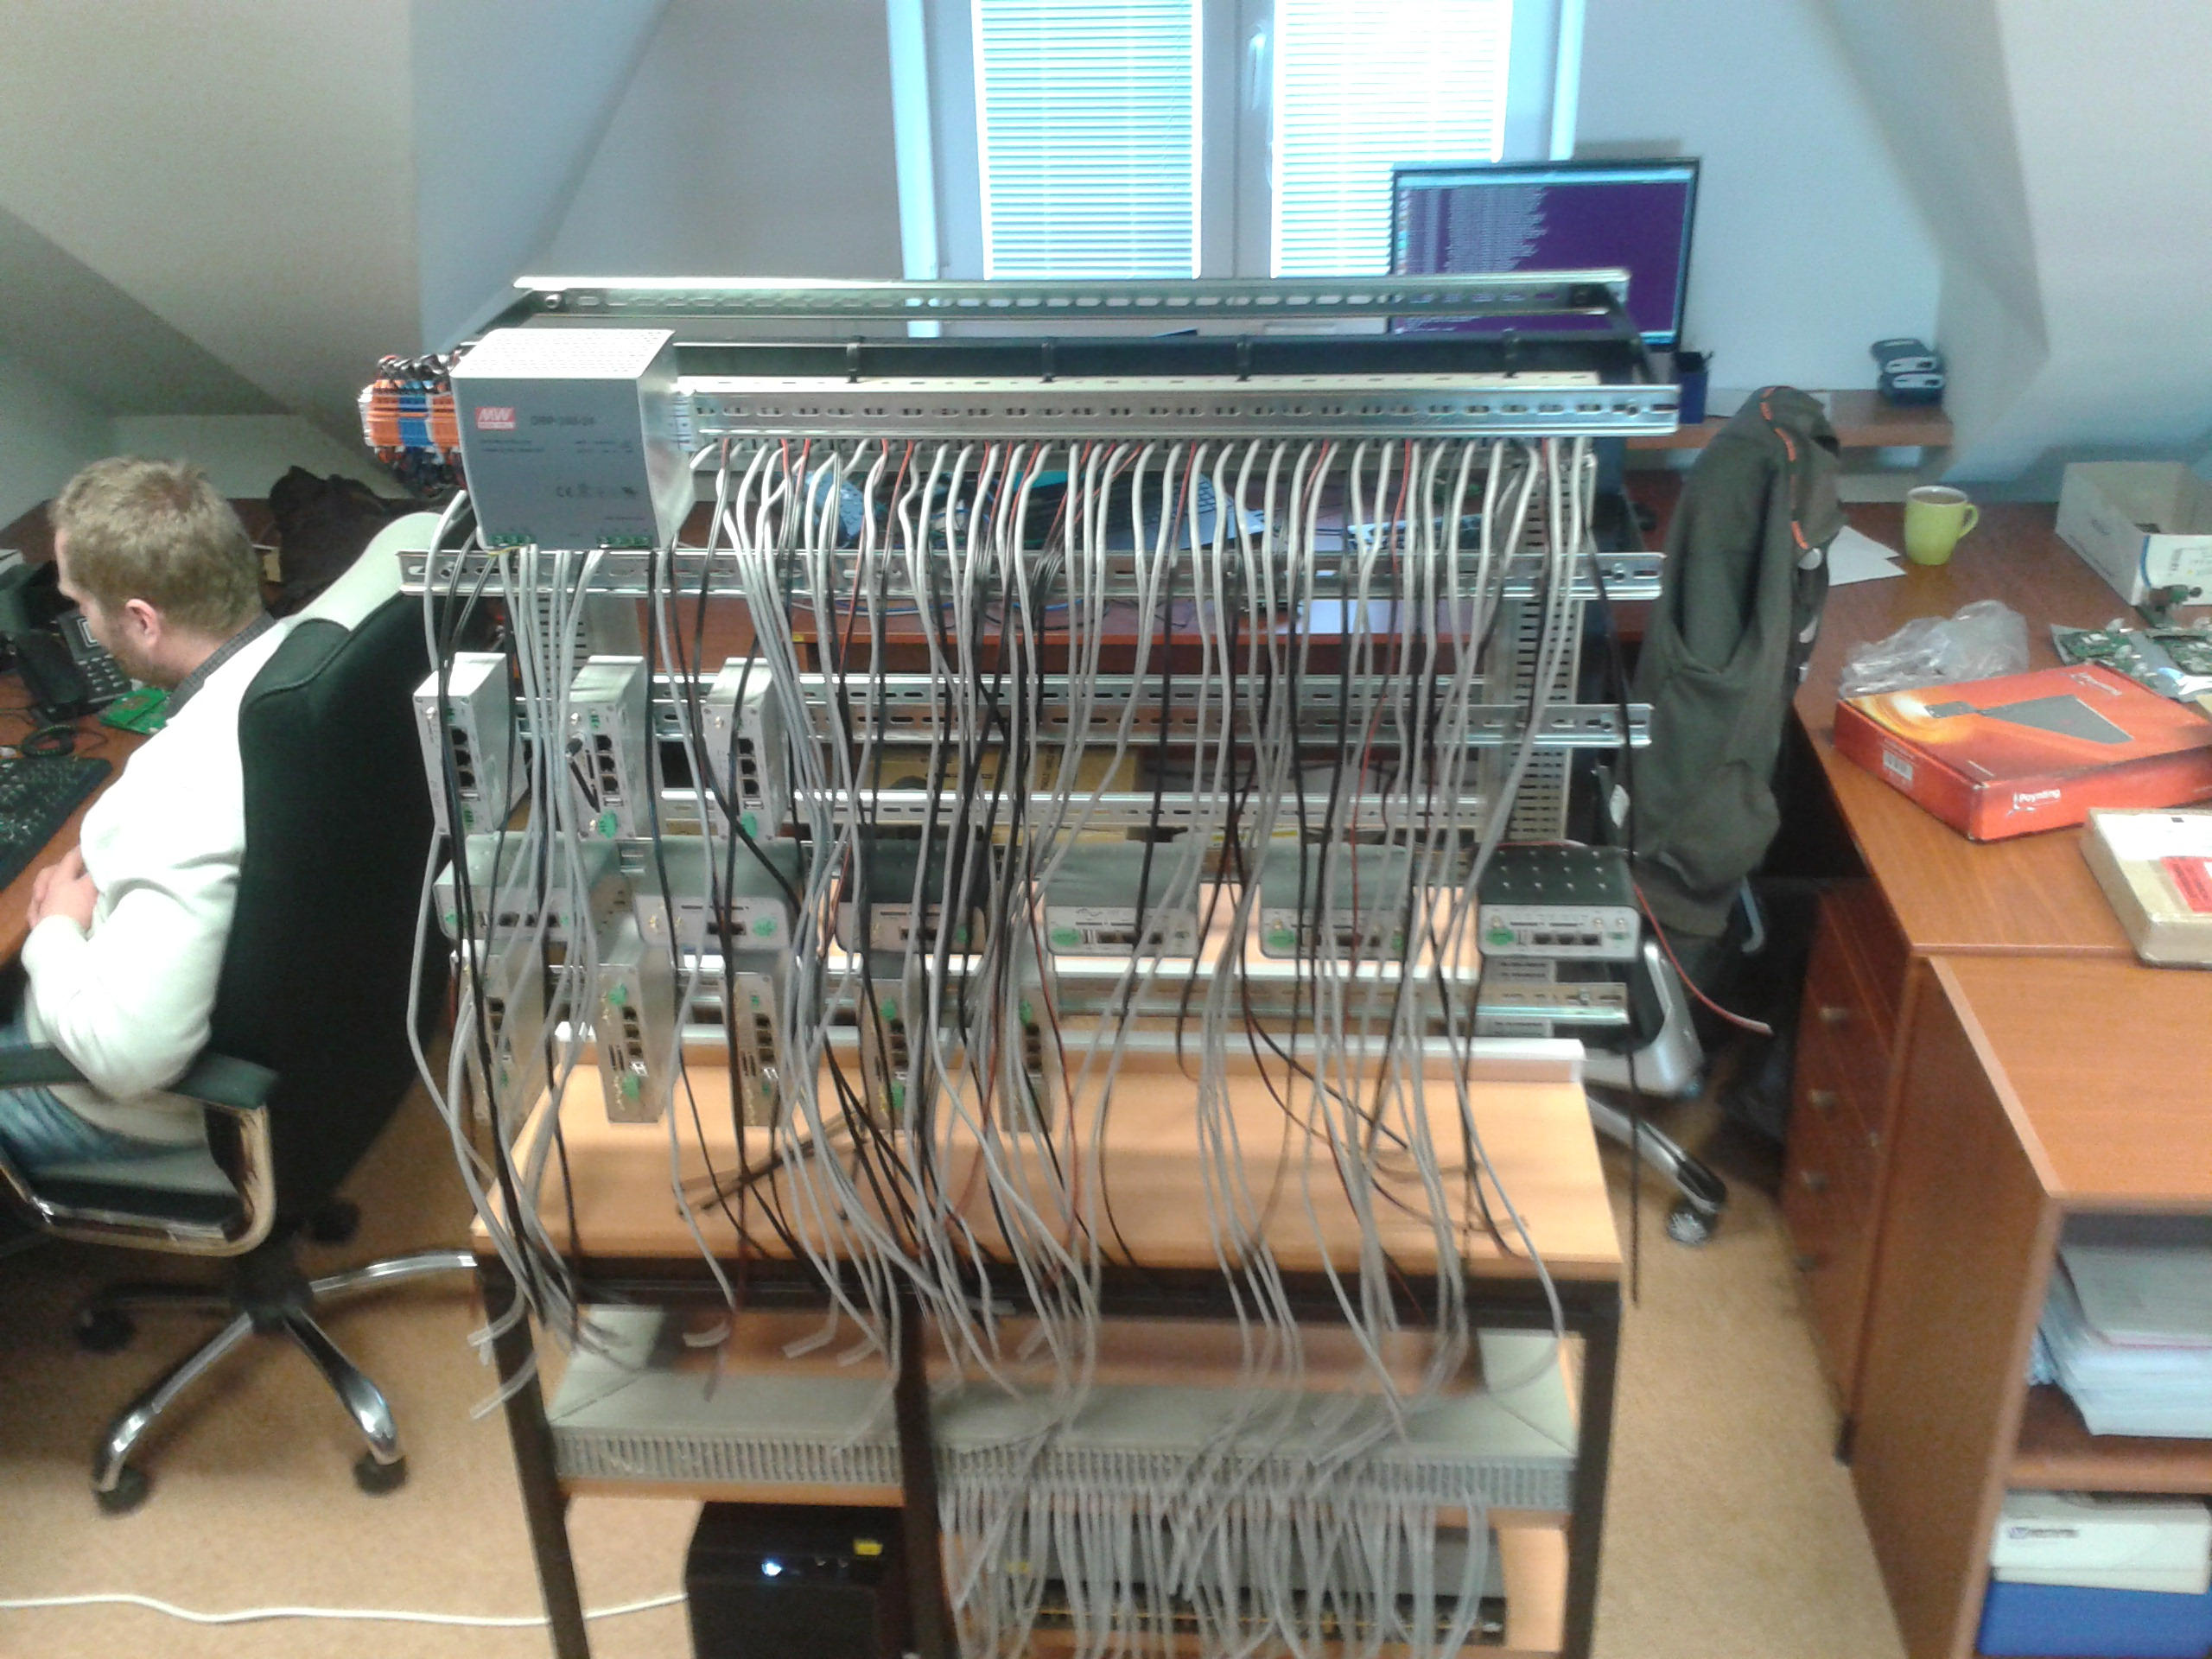
\includegraphics[width=\LW]{stojan2}
  \caption{Příprava kabeláže na stojan}
  \label{fig:stojan2}
\end{figure}

Posledním krokem potřebným pro uvedení testovací laboratoře do~provozu je připojení všech testovaných zařízení. Do~testovací laboratoře jsem zapojil všechny dostupné routery společnosti Conel.

Po zapojení všech testovaných výrobků jsem testovací laboratoř spustil a zahájil testovací provoz, kdy je každý den proveden překlad a test všech výrobků. Při pravidelném testování jsem prozatím nenašel závažné nedostatky. Občasné nepřipojení zařízení do~mobilní sítě je způsobeno velmi slabým signálem v dočasném místě umístění testovacího stojanu. Tento problém by měl být vyřešen přemístěním stojanu po jeho kompletním osazení.

\begin{figure}[h]
  \centering
  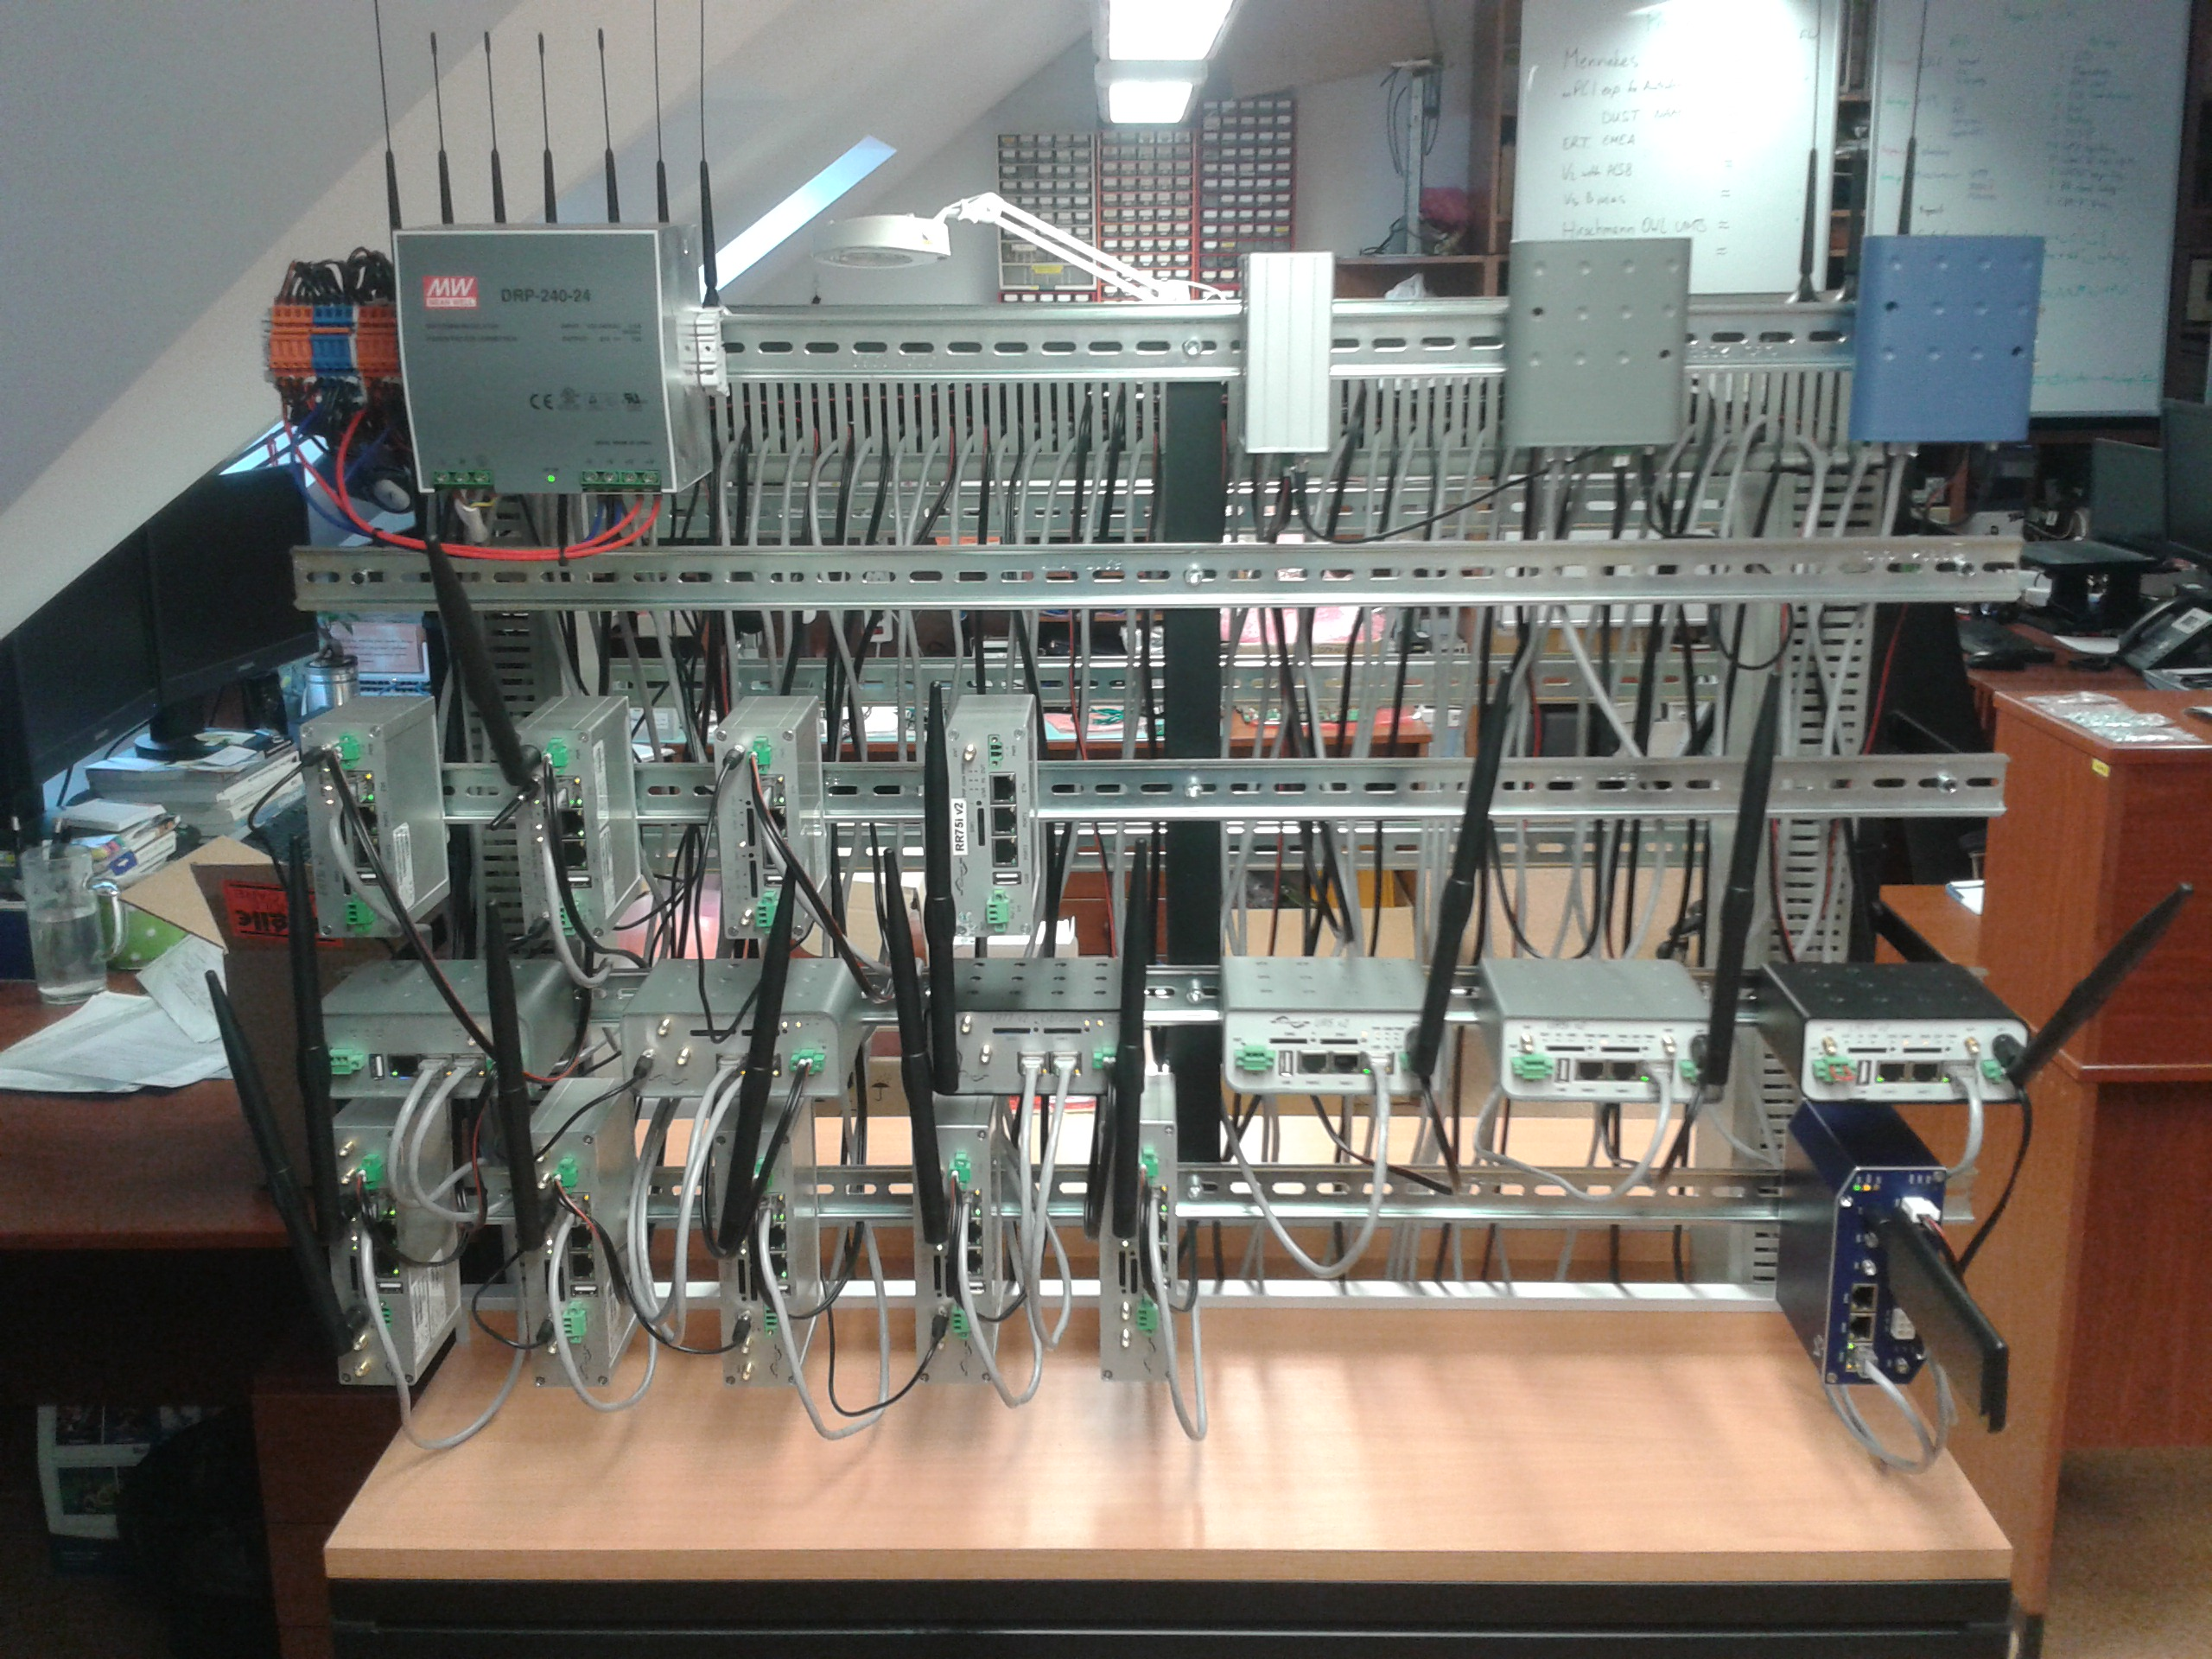
\includegraphics[width=\LW]{stojan4}
  \caption{Dokončené testovací pracoviště}
  \label{fig:stojan4}
\end{figure}

\begin{figure}[h]
  \centering
  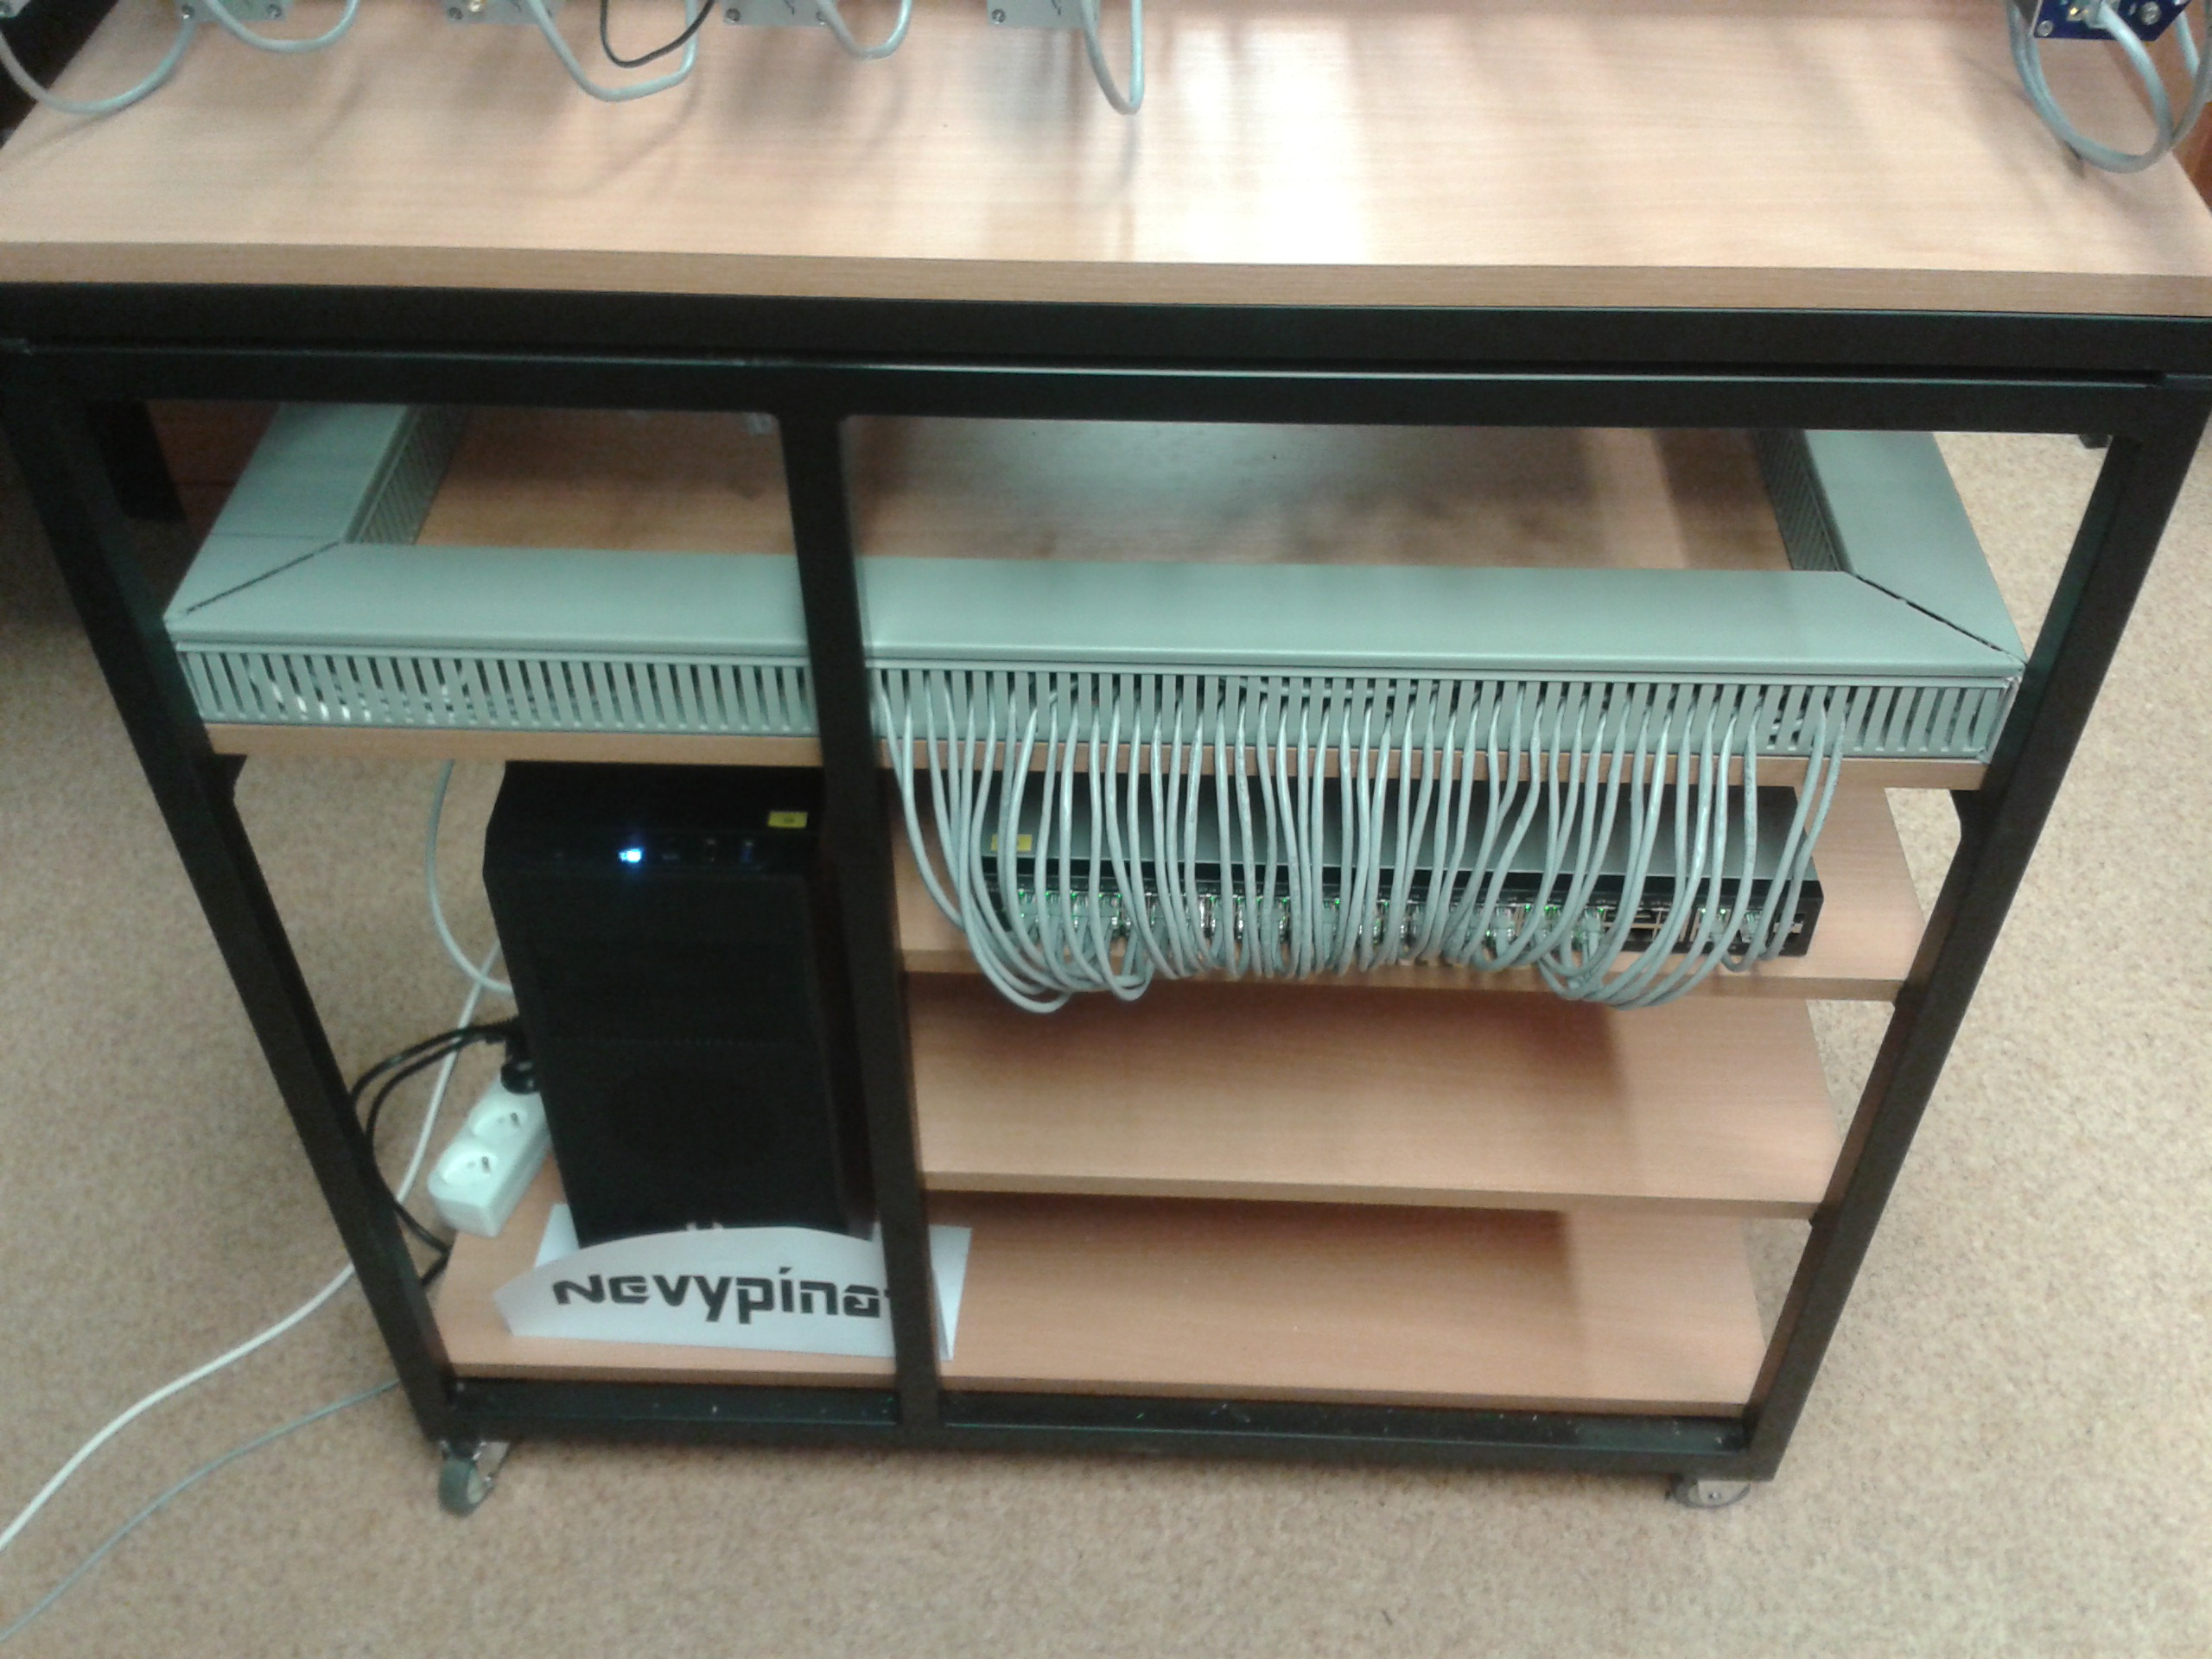
\includegraphics[width=\LW]{stojan3}
  \caption{Dokončené testovací pracoviště}
  \label{fig:stojan3}
\end{figure}



\endinput
